\section{Design}\label{sec:design}
The design has to be as simple as possible, because the more parts there are the more things can go wrong.
% maybe insert quote from elon musk lol
The main problem that one encounters when designing such a system is:
As soon as the motor moves the tube, and with it the player, the other motor cannot rotate the player anymore and vice versa.
To solve this problem, we have to design two parts/systems that can solve this problem.
%The first connects two tubes that can rotate freely but if one moves the other one moves with it.
%The second one is the opposite, it connects two tubes that can move freely back and forth but if one rotates the other one rotates with it.
Therefore, we have two main parts, we called them: Turn Side and Move Side.

\subsection{Move Side}\label{subsec:move-side}
The Move Side is the part that moves the player back and forth.
We use a combination of a gear and a gear rack to move the player, additionally, we have a mechanism that connects the two tubes.
A render of the gears and the gear rack can be seen here:\\
%\begin{figure}[H]
%    \centering
%    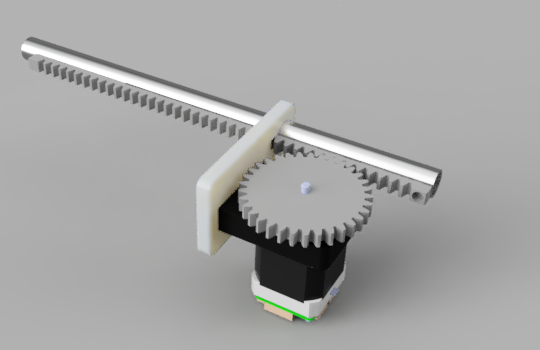
\includegraphics[height=7cm]{../photos/move_side_gear}
%    \caption[moveside1]{Move side gear and gear rack}
%    \label{fig:move_side_gear}
%\end{figure}

\noindent
\begin{tikzpicture}[H]
    \node [anchor=west] (gear) at (-1,3.8) {\Large Gear};
    \node [anchor=west] (gear-rack) at (-1,6) {\Large Gear rack};
    \node [anchor=west, text width=2cm] (motor) at (-1,2) {\Large Motor \small \textbf{(PD42-3-1141)}};
    \node [anchor=east, text width=2cm] (holder) at (18,5) {\Large Holder \small connects the motor to the wall of the table};
    \node [anchor=east, text width=2cm] (tube) at (18,2) {\Large Tube};
    \begin{scope}[xshift=1.5cm]
        \node[anchor=south west,inner sep=0] (image) at (0,0) {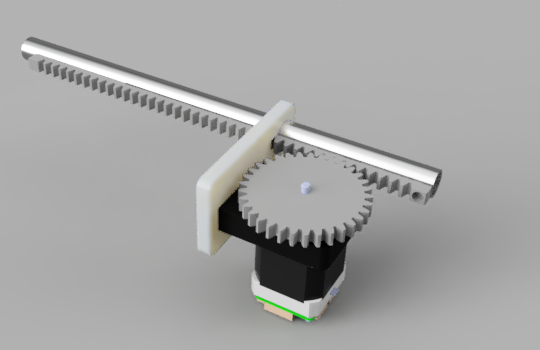
\includegraphics[width=0.7\textwidth]{../photos/move_side_gear}};
        \begin{scope}
            [x={(image.south east)},y={(image.north west)}]
%            \draw[red,ultra thick,rounded corners] (0.48,0.80) rectangle (0.55,0.95);
%            \draw [-latex, ultra thick, red] (note) to[out=0, in=-120] (0.48,0.80);
%            \draw [-stealth, line width=5pt, cyan] (water) -- ++(0.4,0.0);
            \draw [-stealth, line width=2pt, red] (gear) -- ++(0.65, 0.0);
            \draw [-stealth, line width=2pt, red] (motor) -- ++(0.60, 0.0);
            \draw [-stealth, line width=2pt, red] (gear-rack) -- ++(0.40, 0.0);
            \draw [-stealth, line width=2pt, red] (holder) -- ++(-0.67, 0.0);
            \draw [-latex, ultra thick, red] (tube) to[out=180, in=-25] ++(-0.33,0.25);
        \end{scope}
    \end{scope}
\end{tikzpicture}%

% Todo: insert a picture of the meachaism that connects the tubes
\todo{Insert real life image}

\subsection{Turn Side}\label{subsec:turn-side}
The Turn Side is the part that rotates the player.
The turning motor is connected to a tube containing the smaller tube on which the player sits.
The larger tube contains a slit along its length, and the smaller tube has a pin that fits (a screw in this case) into the slit.
A render of the turning mechanism can be seen here:
%\begin{figure}[H]
%    \centering
%    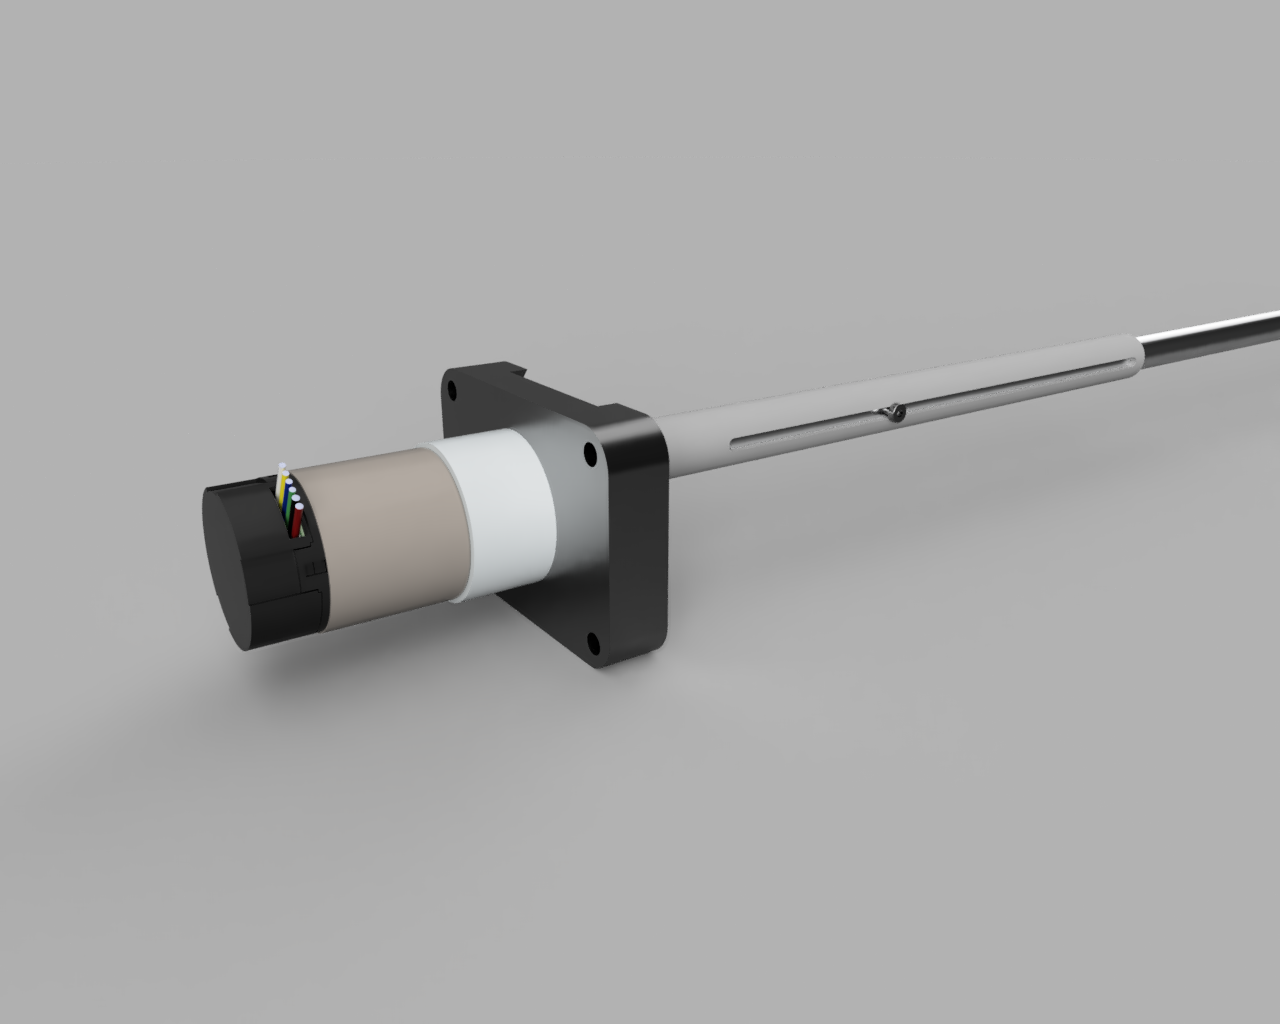
\includegraphics[height=7cm]{../photos/turn_side}
%    \caption[turnside]{Turn side with motor and slit}
%    \label{fig:turn_side2}
%\end{figure}

\noindent
\begin{tikzpicture}[H]
    \node [anchor=west, text width=2cm] (motor) at (-1,5) {\Large Motor \small \textbf{(Pololu)}};
    \node [anchor=east, text width=3cm] (larger-tube) at (18.5,9) {\Large Larger tube \small connected to the motor};
    \node [anchor=east, text width=3cm] (main-tube) at (18.5,7.2) {\Large Main tube \small connected to the player};
    \node [anchor=east, text width=3cm] (slit) at (18.5,5.5) {\Large Slit};
    \node [anchor=east, text width=3cm] (pin) at (18.5,3.5) {\Large Pin};
    \node [anchor=east, text width=3cm] (holder) at (18.5,1.5) {\Large Holder \small connects the motor to the wall of the table};
    \begin{scope}[xshift=1.5cm]
        \node[anchor=south west,inner sep=0] (image) at (0,0) {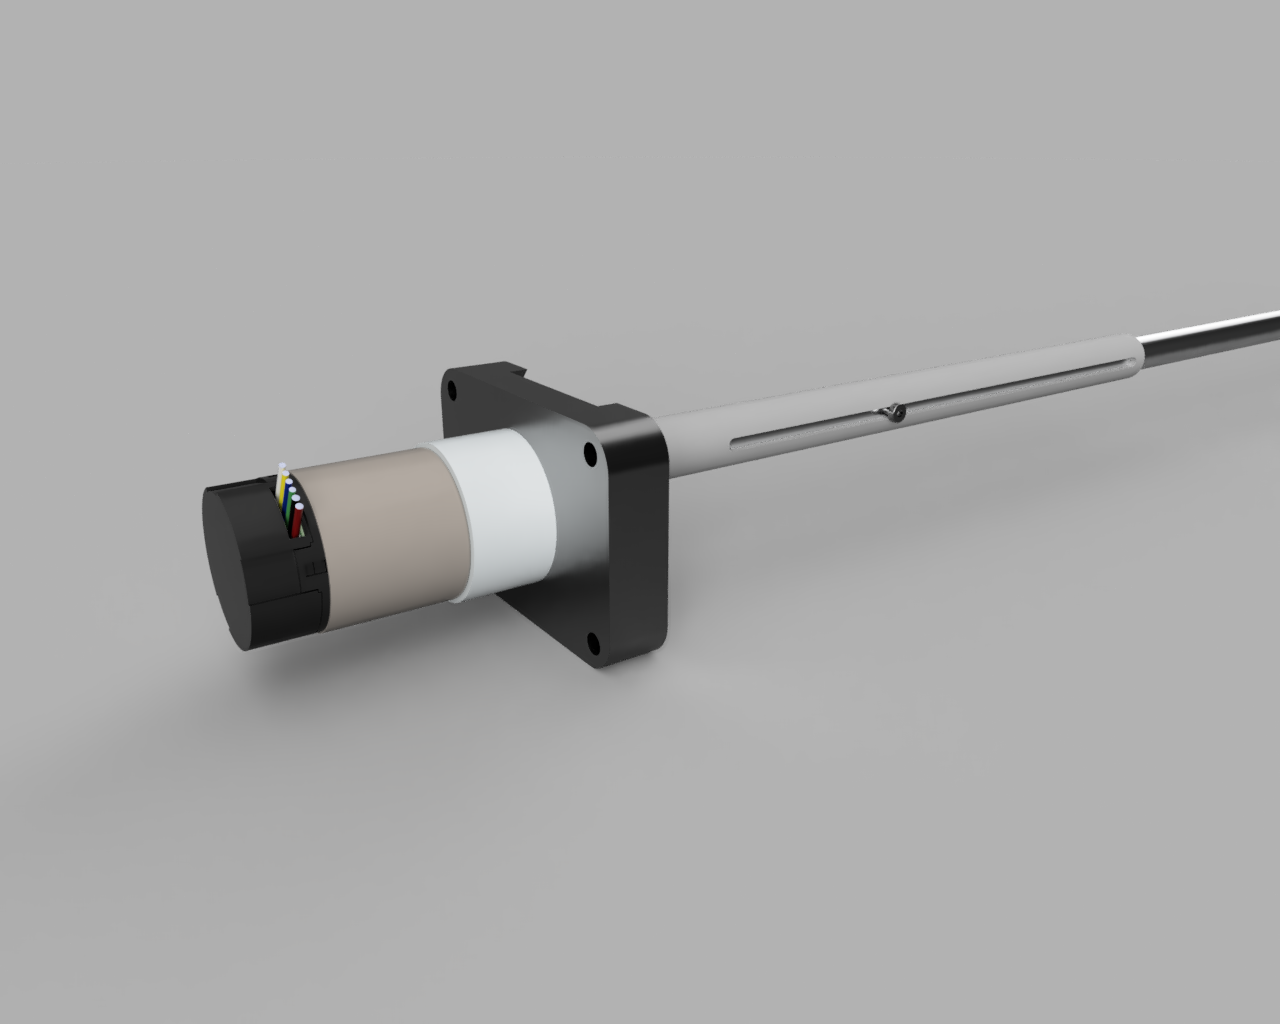
\includegraphics[width=0.7\textwidth]{../photos/turn_side}};
        \begin{scope}
            [x={(image.south east)},y={(image.north west)}]
%            \draw[red,ultra thick,rounded corners] (0.48,0.80) rectangle (0.55,0.95);
%            \draw [-latex, ultra thick, red] (note) to[out=0, in=-120] (0.48,0.80);
%            \draw [-stealth, line width=5pt, cyan] (water) -- ++(0.4,0.0);
            \draw [-stealth, line width=2pt, red] (motor) -- ++(0.25, 0.0);
            \draw [-stealth, line width=2pt, red] (larger-tube) to[out=180, in=90] ++(-0.5, -0.21);
            \draw [-stealth, line width=2pt, red] (main-tube) -- ++(-0.16, 0.0);
            \draw [-stealth, line width=2pt, red] (slit) to[out=180, in=-90] ++(-0.4, 0.1);
            \draw [-stealth, line width=2pt, red] (pin) to[out=180, in=-90] ++(-0.45, 0.265);
            \draw [-stealth, line width=2pt, red] (holder) to[out=180, in=-60] ++(-0.65, 0.2);
%            \draw [-latex, ultra thick, red] (tube) to[out=180, in=-25] ++(-0.33,0.25);
        \end{scope}
    \end{scope}
\end{tikzpicture}%


\todo{Insert real life image}
